\documentclass{article}
\usepackage{amsmath}
\usepackage{amsthm}
\usepackage{amsfonts}
\usepackage{amssymb}
\usepackage{bbold}
\usepackage{dsfont}
\usepackage{graphicx}
\usepackage{cleveref}
\usepackage{bm}
\usepackage{booktabs}
\usepackage{siunitx}
\usepackage{xcolor}
\usepackage{pdfpages}
\usepackage[utf8]{inputenc}
\usepackage[english]{babel}
\newtheorem{definition}{Definition}
\newtheorem{example}{Example}
\newcommand{\exP}[1]{\mathrm{e}^{#1}}
\newcommand{\dif}{\mathrm{d}}
\renewcommand{\vec}[1]{\mathbf{#1}}
\newcommand{\pdagger}{{\phantom{\dagger}}}
\newcommand{\state}[1]{\vert #1\rangle}
\newcommand{\cstate}[1]{\langle #1\vert}
\newcommand{\tr}[1]{\mathrm{tr}\left\{#1\right\}}
\newcommand{\trs}[2]{\, \mathrm{tr}_{#1}\{#2\}}
\newcommand{\expc}[3]{\langle #1\vert #2 \vert #3\rangle}
\usepackage[doi=false,url=false,isbn=false,backend=bibtex,style=nature,natbib=true,sorting=none]{biblatex}
\bibliography{bib.bib}
\usepackage{geometry}
\geometry{
	a4paper,
	total={170mm,257mm},
	left=15mm,
	right=15mm,
	top=15mm,
}
\begin{document}
\title{spin-PLDM: Derivation}
%\author{Rudolf Smorka}
\maketitle
Summary based on \cite{mannouch2020partially}.
\section{Fully vs partially linearized methods}
\subsection{Fully linearized methods}
\begin{itemize}
	\item Fully linearized methods result from performing a linearization approximation to the difference between the forward and backward paths for \textbf{both the electronic and nuclear degrees of freedom}; a semiclassical approximation that is expected to be valid in the classical limit.
	\item When applied to fully electronic system, this approximation is exact.
	\item When there is electron-nuclear coupling, it consists an additional approximation (additional, in the sense, that mapping itself is already an approximation).
\end{itemize}
\subsection{Partially linearized methods}
\begin{itemize}
	\item Perform linearization approximation for nuclear paths and then treat dynamics of forward and backward electronic paths separately. 
	\item Hope that this improves linearized method
	\item Often, partially linearized methods are better than their fully linearized counterparts
	\item PLDM first introduced for the MMST mapping by Coker and Huo in 2010s. Spin-PLDM first introduced by Jonathan and Jeremy in 2020. Spin-PLDM also has been shown to give better results in the spin-boson model and the FMO model than other mapping-based approaches.
\end{itemize}
\subsection{How it fits into the picture}
\begin{figure}[!h]
	\centering
	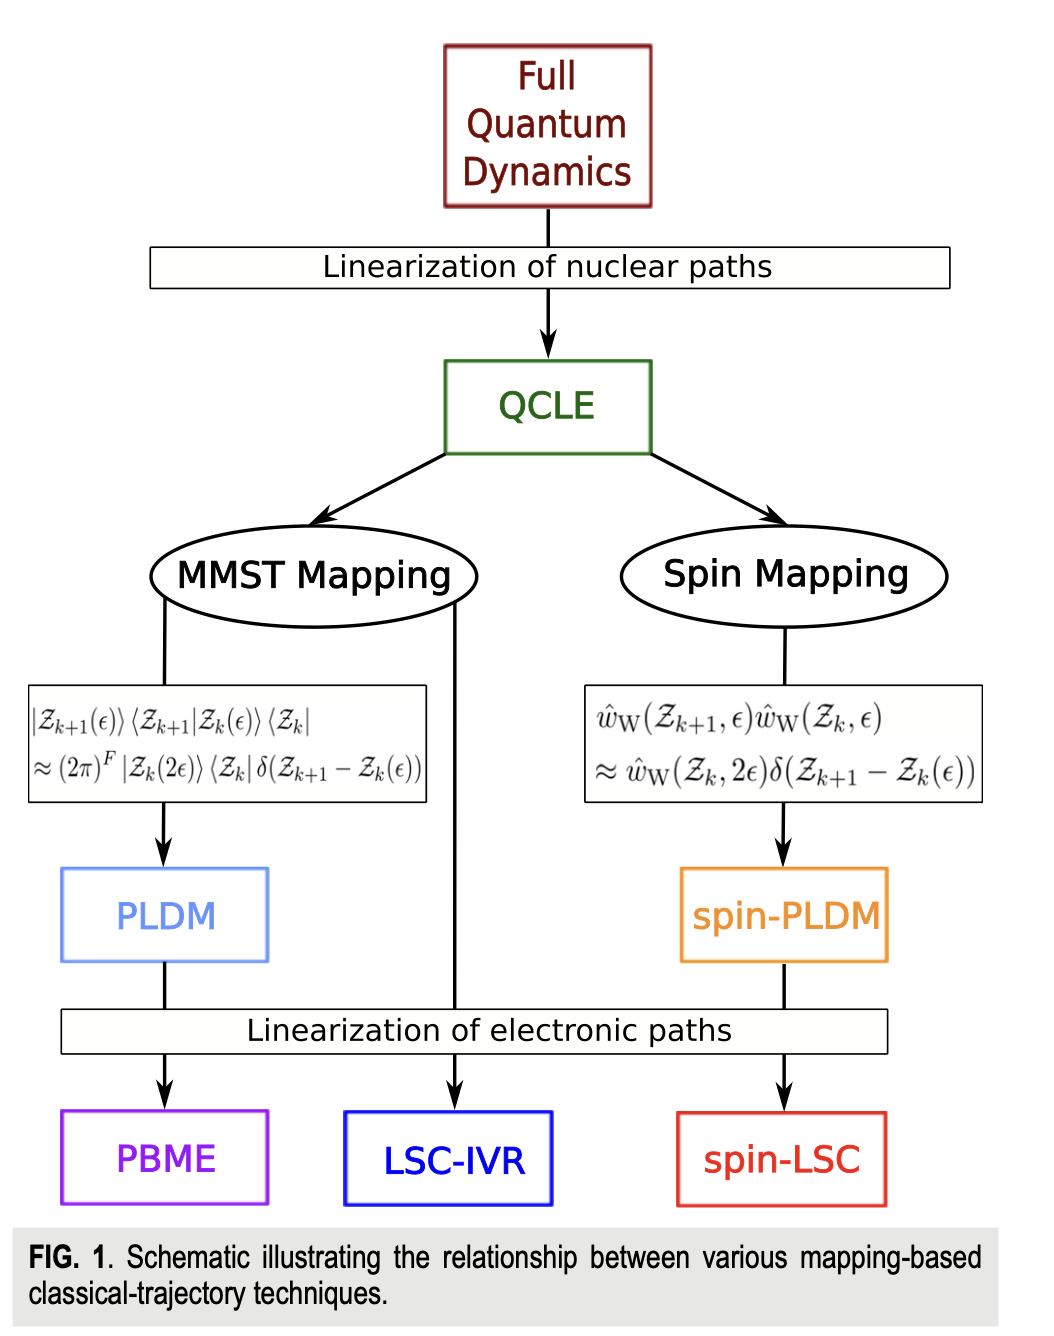
\includegraphics[width=0.35\textwidth]{figs/scheme.png}
\end{figure}
\clearpage
\section{Theory}
\subsection{Model}
A nuclear-electron coupled quantum-classical system is considered:
\begin{equation}
	H = \frac{p^2}{2m} + V_0(x) + V(x).
\end{equation}
Here, $V_0(x)$ is the state-independent potential, and $V(x)$ the state-dependent potential. As usual, the nuclei are assumed to be classical and the electrons are quantum mechanical.
One partitions the potential energy such that $\tr{V(x)}=0$ (the trace is over the electronic subsystem).

One is interested in correlation functions
\begin{align}
	C_{AB}(t) &= \mathrm{Tr}\{\rho_0 A_0B(t)\}\\
	&\equiv \mathrm{Tr}\{\rho_\mathrm{b} A\exP{iHt}B\exP{-iHt}\}.
\end{align}
Here, what happened from line 1 to 2 are a couple of things: 1) The initial state is assumed to be factorized $\rho_0 = \rho_\mathrm{b}(0) \rho_\mathrm{el}(0)$, 2) the operator $A=\rho_\mathrm{el}(0)A_0$ initializes the electronic subsystem, and 3) we used Heisenberg-evolution of operator $B(t)$. One can, in principle, lift the assumption of a initially factorized state, by definition $A = \sum_j \rho_\mathrm{el}^{(j)}A^{(j)}_0$.

Next, we insert completeness relation for the electronic basis $\vert \lambda\rangle$ and nuclear basis $\vert x_0 \rangle $
\begin{align}
	C_{AB}(t) &= \sum_{\lambda,\lambda'}\sum_{\mu,\mu'} \langle \lambda \vert A\vert \lambda'\rangle\langle \mu'\vert B\vert \mu\rangle \int \dif x_0 \dif x'_0 \dif x_N \langle x_0 \vert \rho_b \vert x_0'\rangle \langle \lambda',x'_0\vert \exP{iHt}\vert \mu',x_N\rangle\langle \mu,x_N\vert \exP{-iHt}\vert \lambda,x_0\rangle.\\
\end{align}
The ordering has a logic behind it: The unprimed variables are for forward propagation, the primed for backward propagation. Also, $x_N=x'_N$, because there is no nuclear operator applied at time $t$. It has been added just to be symmetric.

Next, one does a linearization approximation. This is to avoid sampling complex phases for the nuclear degrees of freedom. This approximation is the main point for treating the dynamics of the nuclei classically. To do so, one first transforms the nuclear variables into sums and differences
\begin{equation}
	\bar{x}_k = \frac{1}{2}(x_k +x'_k), \qquad \Delta x = x_k - x'_k,
\end{equation}
where $x_k$ is the nuclear coordinate in the path integral step $k$. The approximation is then retaining all terms up to first order in $\Delta x_k$. One then gets the approximate correlation function
\begin{equation}
	C_{AB}(t) \approx \sum_{\lambda,\lambda'}\sum_{\mu,\mu'} \langle \lambda \vert A\vert \lambda'\rangle\langle \mu'\vert B\vert \mu\rangle \int \dif \bar{x}_0 \dif \bar{p}_0 \rho_b(\bar{x}_0,\bar{p}_0)\int \frac{\dif \Delta \bar{p}_0}{(2\pi)^f}\dif \bar{x}_N\prod_{k=1}^{N-1}\dif \bar{x}_k\frac{\dif \bar{p}_k}{(2\pi)^f}\dif \Delta x_k\frac{\dif \Delta p_k}{(2\pi)^f} T'_{[\lambda',\mu']}T_{[\mu,\lambda]}\exP{i\Delta S_0}.
\end{equation}


\subsection{Partially linearized density matrix}
\subsection{spin-mapping Partially linearized density matrix}

\printbibliography
\end{document}


